\begin{frame}
\frametitle{Depth Buffer: Demo}

\begin{columns}

\column{.5\textwidth}

\begin{figure}[ht]
    \centering
    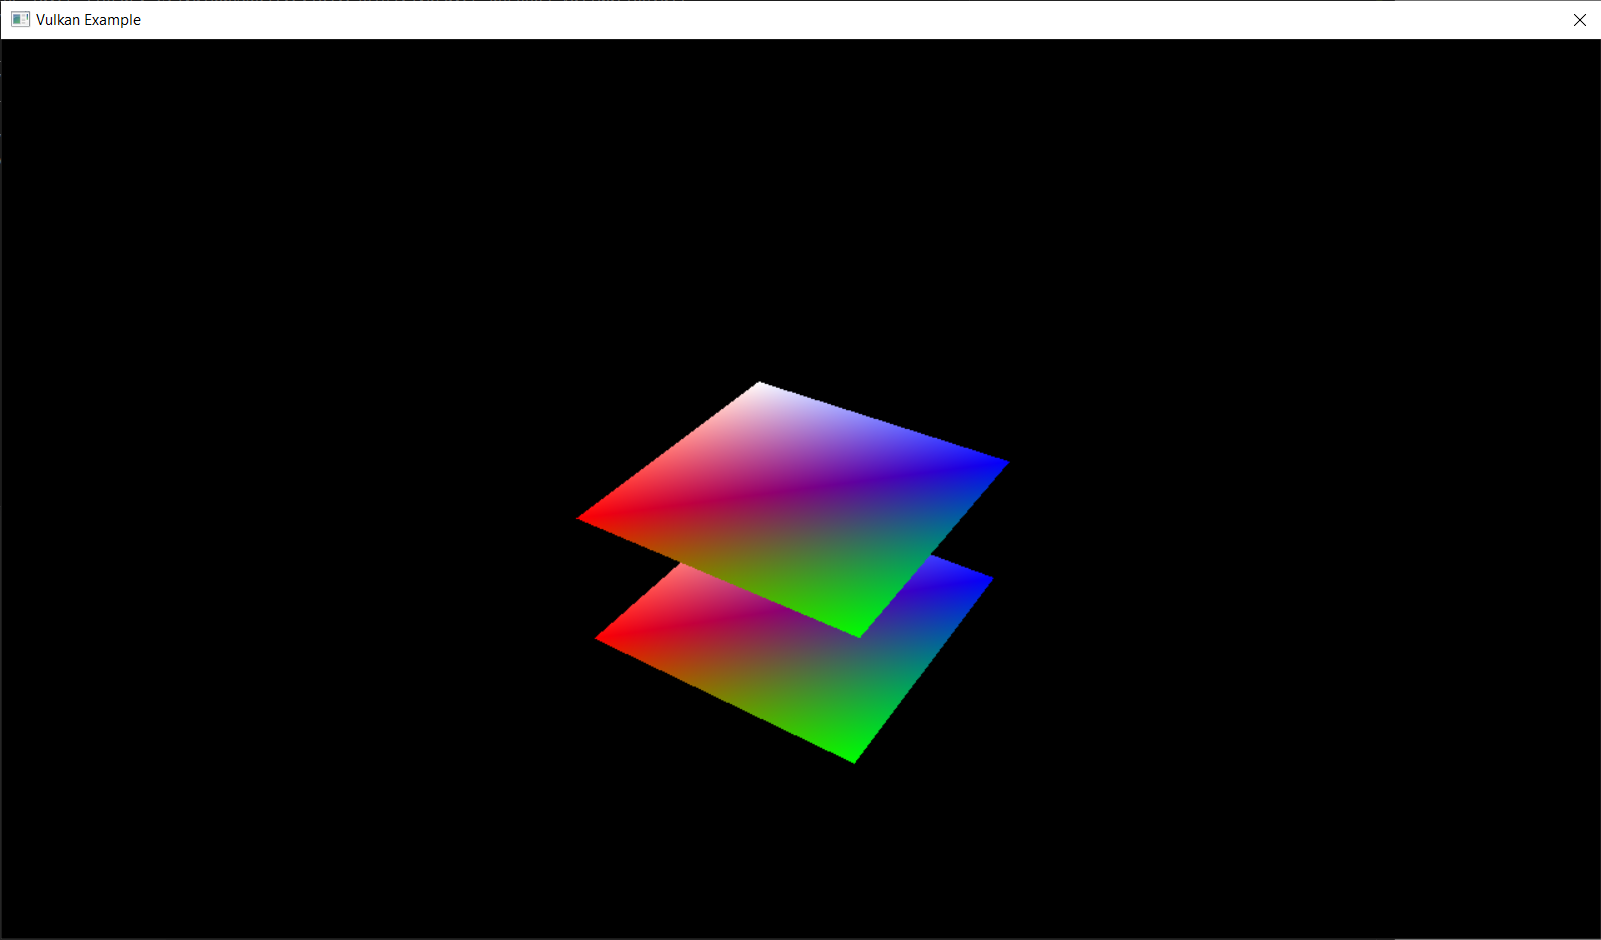
\includegraphics[scale=0.14]{images/SlidesDepthTesting/DepthTesting.png}
\end{figure}

\column{.5\textwidth}

\begin{figure}[ht]
    \centering
    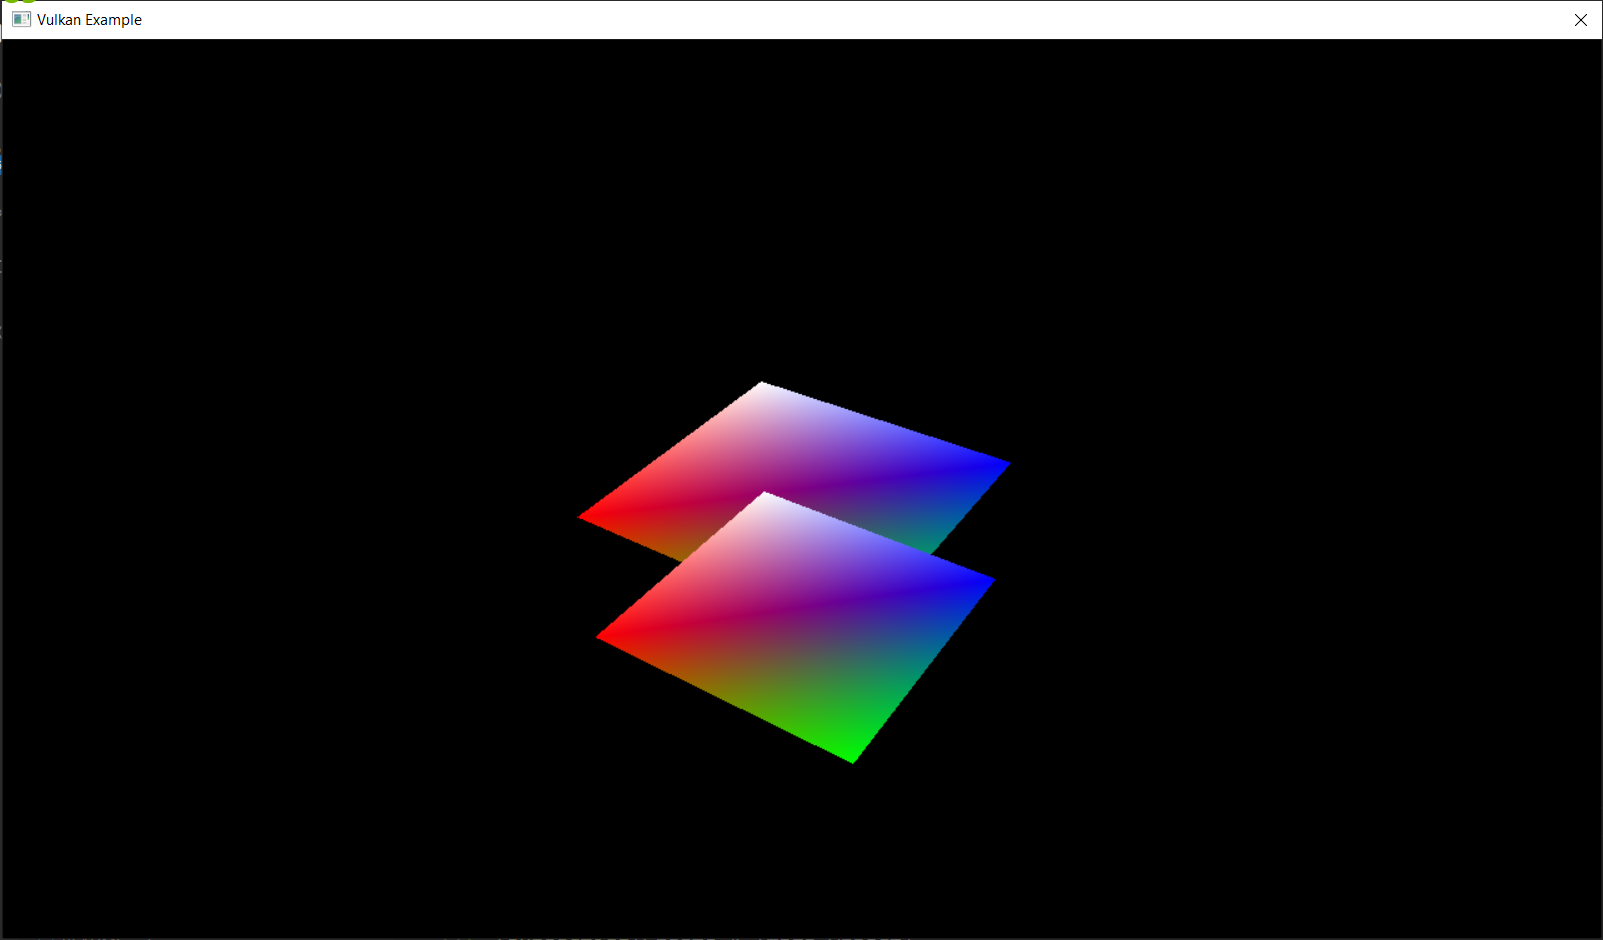
\includegraphics[scale=0.14]{images/SlidesDepthTesting/NoDepthTesting.png}
\end{figure}

\end{columns}

\end{frame}

\begin{frame}
\frametitle{Depth Buffer}
\begin{itemize}
\item Come renderizzare oggetti in modo tale che quelli più vicini possano nascondere quelli più lontani?
\item Possiamo ordinare gli oggetti in base alla loro lontananza dalla camera
\item E se due oggetti si sovrappongono?
\item Se gli oggetti da renderizzare sono opachi, usiamo un depth buffer
\item Un depth buffer è un'immagine che codifica informazioni riguardanti la profondità dei frammenti
\item Quando un frammento viene generato, compariamo la sua profondità con quella salvata nel corrispettivo texel del depth buffer
\item Se è più grande, il frammento non viene ignorato
\item Se è più piccola, il frammento viene utilizzato e la sua profondità viene salvata nel depth buffer
\item Creiamo un'immagine da usare come depth stencil attachment
\item Abilitiamo il depth testing quando creiamo il pipeline state object
\end{itemize}
\end{frame}
